\documentclass[conference]{IEEEtran}
\IEEEoverridecommandlockouts
\usepackage{cite}
\usepackage{amsmath,amssymb,amsfonts}
\usepackage{graphicx}
\usepackage{textcomp}
\usepackage{xcolor}
\usepackage{booktabs}
\usepackage{multirow}
\usepackage{url}
\usepackage[T1]{fontenc}
\usepackage{lmodern}
\usepackage{microtype}
\usepackage{tikz}
\usetikzlibrary{positioning,arrows.meta,fit,backgrounds}
\usepackage{listings}
\lstset{
  basicstyle=\ttfamily\scriptsize,
  breaklines=true,
  frame=single,
  frameround=tttt,
  belowskip=0pt,
  aboveskip=4pt
}

\begin{document}

\title{SensorWF: A FAIR Generalizable Workflow Framework\\for Multi-Domain Scientific Time-Series Analysis}

\author{
  \IEEEauthorblockN{Author Name\textsuperscript{1},
                    Author Name\textsuperscript{2}}
  \IEEEauthorblockA{\textsuperscript{1}\textit{Department, Institution, City, Country}\\
                    \textsuperscript{2}\textit{Department, Institution, City, Country}\\
                    email@example.com}
}

\maketitle

\begin{abstract}
Scientific sensor data pervades disciplines from spacecraft engineering and clinical
medicine to atmospheric science---and in each case, the analytical pipeline follows
the same skeleton: ingest raw archives, assess quality, engineer features, annotate
semantically, and record provenance. Yet these pipelines are routinely published as
monolithic, domain-specific scripts whose assumptions remain implicit and whose
components resist reuse across disciplinary boundaries.
We present \textbf{SensorWF}, a FAIR-annotated workflow framework for generalizable
scientific time-series analysis. A five-module reusable core (M1--M5) with typed
I/O contracts forms the analytical backbone; a \emph{domain adapter} pattern confines
all domain-specific logic to M1 so that M2--M5 execute identically across disciplines,
encoding domain assumptions in a machine-readable component registry so that any
sensor domain can be integrated and reused without altering the analytical core.
Domain-specific analyses attach as \emph{use-case extensions} without modifying the
core. Runtime PROV-O/ProvONE provenance traces---including SHA-256 checksums for all
file-path entities---and SSN/SOSA-aligned OWL ontologies are emitted as first-class
outputs. To validate generalizability, we instantiate SensorWF across three
scientifically distinct domains---spacecraft telemetry, ambulatory ECG, and
atmospheric climate---and demonstrate synthetic fault injection and multi-detector
anomaly detection as a representative use-case extension. Results confirm that a
single codebase, parameterised solely through M1 adapters of approximately 150 lines
each, supports complete analytical pipelines across domains with markedly different
sampling rates, channel counts, and fault taxonomies. All code, component registry,
ontology artefacts, and datasets are released as an open scientific object.
\end{abstract}

\begin{IEEEkeywords}
computational workflows, FAIR principles, domain adaptation, sensor analytics,
anomaly detection, PROV-O, ProvONE, knowledge graph, reproducibility
\end{IEEEkeywords}

%% =========================================================
\section{Introduction}
\label{sec:intro}
%% =========================================================

Sensor-driven scientific disciplines share a computational burden that receives
little formal architectural attention. Raw measurements must be ingested, corrected
for artefacts, and transformed into analysis-ready feature representations---each
stage encoding domain assumptions about sampling rates, quality thresholds, and
channel semantics that are seldom made explicit or machine-readable. Downstream
analyses then layer further domain-specific logic on top of this shared skeleton.

Despite this structural commonality, pipelines across domains are almost universally
developed in isolation as monolithic, domain-specific scripts. The resulting
fragmentation prevents reuse, makes cross-domain comparisons unreliable, and renders
post-publication audit practically impossible. The eScience and open-science
communities have called for pipelines to be treated as first-class scientific
objects whose provenance can be traced, shared, and reused
\cite{wilkinson2016fair,garijo2022fair}.

This paper presents \textbf{SensorWF} (\emph{Generalizable FAIR Sensor Analytics
Workflow}), a framework for multi-domain scientific sensor time-series analysis.
The five-module core handles ingestion (M1), quality assessment (M2), feature
engineering (M3), semantic annotation (M4), and provenance export (M5).
Domain-specific analysis tasks attach as \emph{use-case extensions}: we demonstrate
synthetic fault injection (E1) and automated anomaly detection (E2).
Fig.~\ref{fig:architecture} illustrates the full architecture.
The paper makes four specific contributions:

\begin{enumerate}
  \item \textbf{A generalizable five-module core} (M1--M5) with typed
    I/O contracts and explicit scientific assumptions. The \emph{domain adapter}
    pattern isolates domain-specificity in M1; M2--M5 execute identically across
    disciplines via adapter-supplied configuration.
  \item \textbf{A machine-readable component registry} (\texttt{components.json})
    encoding domain assumptions as typed ports, configuration parameters, domain
    tags, and ProvONE URIs for every module---so that any sensor domain can be
    integrated and reused without altering the analytical core---enabling automated
    composition, discovery, and extension.
  \item \textbf{Runtime provenance and semantic annotation.} SensorWF emits
    PROV-O/ProvONE Turtle provenance for every execution---including SHA-256
    checksums for all file-path entities---and maps analytical evidence to domain
    OWL ontologies (SSN/SOSA-aligned \cite{compton2012ssn}),
    producing SPARQL-queryable knowledge graphs.
  \item \textbf{Cross-domain validation via an anomaly detection use case.}
    We demonstrate SensorWF across three well-established datasets using E1 fault
    injection and E2 multi-detector evaluation as a concrete analytical extension.
\end{enumerate}

%% ── Fig 1: Architecture (double-column TikZ) ──────────────────────────────────
\begin{figure*}[t]
\centering
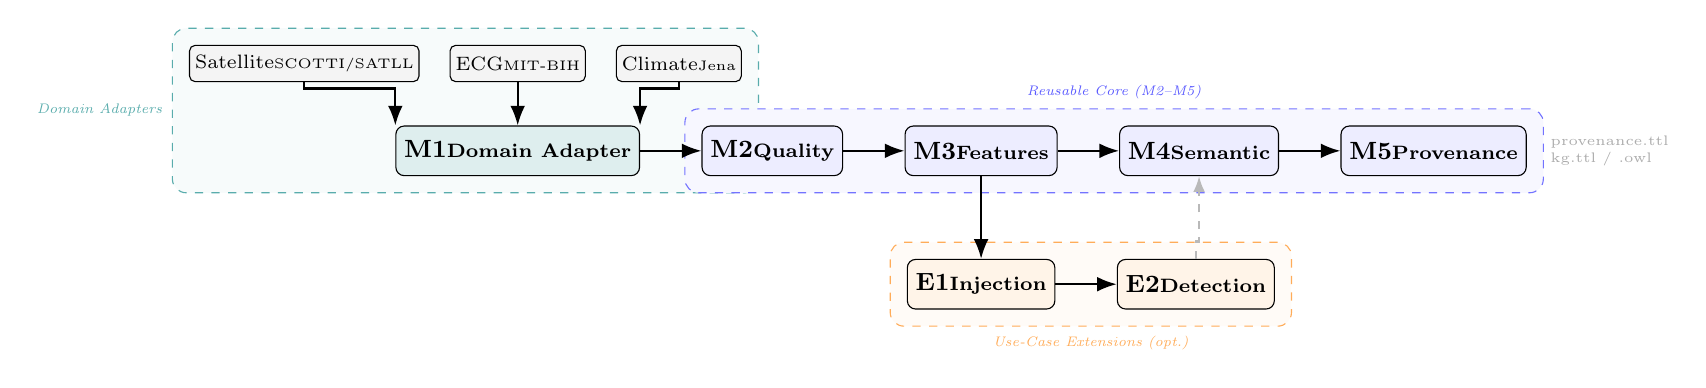
\begin{tikzpicture}[
  box/.style={draw, rounded corners=3pt, minimum width=1.65cm, minimum height=0.63cm,
              text centered, font=\small\bfseries, fill=white, inner sep=3pt},
  src/.style={draw, rounded corners=2pt, minimum width=1.25cm, minimum height=0.46cm,
              text centered, font=\scriptsize, fill=gray!9, inner sep=2pt},
  ext/.style={draw, rounded corners=3pt, minimum width=1.65cm, minimum height=0.63cm,
              text centered, font=\small\bfseries, fill=orange!9, inner sep=3pt},
  arr/.style={-{Latex[length=2.5mm]}, thick},
  darr/.style={-{Latex[length=2mm]}, thick, dashed, gray!55},
  node distance=0.5cm and 0.78cm
]
%% Data sources (top row)
\node[src] (dsrc1) {Satellite\\\tiny SCOTTI/SATLL};
\node[src, right=0.38cm of dsrc1] (dsrc2) {ECG\\\tiny MIT-BIH};
\node[src, right=0.38cm of dsrc2] (dsrc3) {Climate\\\tiny Jena};

%% M1 domain adapter (below sources, centred)
\node[box, below=0.55cm of dsrc2, fill=teal!13] (nm1)
  {M1\\\scriptsize Domain Adapter};
\draw[arr] (dsrc1.south) -- ++(0,-0.08) -| (nm1.north west);
\draw[arr] (dsrc2.south) -- (nm1.north);
\draw[arr] (dsrc3.south) -- ++(0,-0.08) -| (nm1.north east);

%% Core processing modules (horizontal chain right of M1)
\node[box, right=0.78cm of nm1, fill=blue!7] (nm2) {M2\\\scriptsize Quality};
\node[box, right=0.78cm of nm2, fill=blue!7] (nm3) {M3\\\scriptsize Features};
\node[box, right=0.78cm of nm3, fill=blue!7] (nm4) {M4\\\scriptsize Semantic};
\node[box, right=0.78cm of nm4, fill=blue!7] (nm5) {M5\\\scriptsize Provenance};

\draw[arr] (nm1) -- (nm2);
\draw[arr] (nm2) -- (nm3);
\draw[arr] (nm3) -- (nm4);
\draw[arr] (nm4) -- (nm5);

%% Use-case extensions (below M3 and M4)
\node[ext, below=1.05cm of nm3] (ne1) {E1\\\scriptsize Injection};
\node[ext, right=0.78cm of ne1] (ne2) {E2\\\scriptsize Detection};

\draw[arr] (nm3.south) -- ++(0,-0.26) -- (ne1.north);
\draw[arr] (ne1) -- (ne2);
\draw[darr] (ne2.north) -- ++(0,0.22) -| (nm4.south);

%% Output artifact label
\node[font=\tiny, right=0.18cm of nm5, align=left, text=gray!65]
  {provenance.ttl\\kg.ttl / .owl};

%% Background region annotations
\begin{scope}[on background layer]
  \node[draw=teal!65, dashed, rounded corners=5pt, fill=teal!3, inner sep=6pt,
        fit={(dsrc1)(dsrc2)(dsrc3)(nm1)},
        label={[font=\tiny\itshape,text=teal!65]left:Domain Adapters}] {};
  \node[draw=blue!55, dashed, rounded corners=5pt, fill=blue!3, inner sep=6pt,
        fit={(nm2)(nm3)(nm4)(nm5)},
        label={[font=\tiny\itshape,text=blue!65]above:Reusable Core (M2--M5)}] {};
  \node[draw=orange!65, dashed, rounded corners=5pt, fill=orange!3, inner sep=6pt,
        fit={(ne1)(ne2)},
        label={[font=\tiny\itshape,text=orange!65]below:Use-Case Extensions (opt.)}] {};
\end{scope}
\end{tikzpicture}
\caption{SensorWF architecture. The domain adapter (teal, M1) normalises raw
         sensor archives from three domains into a standardised DataFrame. The
         reusable core (blue, M2--M5) performs quality assessment, feature
         engineering, semantic annotation, and provenance export identically
         across all domains. Optional use-case extensions (orange, E1--E2) inject
         synthetic faults and evaluate ML detectors; E2 results optionally enhance
         M4's knowledge graph (dashed arrow). Switching domains requires only a new
         M1 adapter ($\approx$150\,lines of Python); M2--M5 require no modification.}
\label{fig:architecture}
\end{figure*}

%% =========================================================
\section{Background and Related Work}
\label{sec:background}
%% =========================================================

\subsection{FAIR Computational Workflows}

The FAIR principles---Findable, Accessible, Interoperable, Reusable---were
originally formulated for scientific data \cite{wilkinson2016fair} and subsequently
extended to computational workflows \cite{garijo2022fair}. FAIR workflows expose
typed module specifications, machine-readable provenance, and explicit scientific
assumptions. Mitchell et al.\ \cite{mitchell2022fair} demonstrate PROV-O
provenance for epidemiological pipelines. WorkflowHub \cite{wilkinson2025workflowhub}
operationalises workflow registration and RO-Crate packaging. Rossi et al.\
\cite{rossi2025openeo} integrate provenance into the openEO Earth Observation
platform. SensorWF complements these efforts by targeting
\emph{multi-domain generalizability} through a structured adapter pattern and a
machine-readable component registry.

\subsection{Domain Adapter Patterns in Scientific Computing}

Separating domain-specific components from reusable algorithmic cores is
well-established in scientific computing---the Galaxy platform
\cite{afgan2018galaxy} and time-series toolkits such as TSFEL \cite{barandas2020tsfel}
are representative examples. SensorWF formalises this separation as an explicit
architectural invariant: M1 is the sole domain-varying component, while M2--M5
consume a standardised DataFrame schema regardless of origin. Portability
boundaries---e.g., M2 assumes temporally regular sampling; irregular-rate streams
require additional extensions---are documented as \texttt{sensorwf:hasAssumption}
predicates in the component registry.

\subsection{Anomaly Detection Benchmarks and Methods}

For spacecraft telemetry, Hundman et al.\ \cite{hundman2018detecting} established
LSTM-based detection on NASA SMAP/MSL. The OPS-SAT benchmark
\cite{ruszczak2025opssat} provides segment-level ground truth and evaluates
dynamic non-parametric thresholding; the ESA Anomaly Database (ESA-ADB)
\cite{esa_adb2024} provides event-level ground truth with affiliation-aware
and range-based metrics that more accurately reflect operational use than
point-wise AUC-ROC. SensorWF's E2 currently uses static EVT-calibrated thresholds
for density-based detectors; full adoption of event-wise metrics and dynamic
postprocessing is a priority extension.

For biomedical ECG, the MIT-BIH Arrhythmia Database \cite{moody2001mitbih} is
the canonical benchmark for arrhythmia detection \cite{kachuee2018ecgclass}. For
climate data, the Jena Climate Dataset \cite{jena_climate} is widely studied with
autoregressive and isolation-based methods \cite{martinez2020climate}. Wu and
Keogh \cite{wu2022benchmarks} demonstrate that single-axis difficulty scaling
produces misleading detector rankings, motivating E1's simultaneous scaling of
amplitude, duration, and channel spread.

Recent competitive baselines include transformer architectures such as
iTransformer \cite{itransformer2024} and TranAD \cite{tuli2022tranad},
and the adaptive ensemble RAMSeS \cite{ramses2026}; robust VAE variants
RVAE-ST \cite{rvaest2025} and STREAM-VAE \cite{streamvae2025} are directly
compatible with E2's detector registry. Conditional attribution methods
\cite{condattrib2026} could augment M4's ontology mapping with context-aware
explanations. SensorWF's E2 and M4 registries accommodate these extensions
without modifying M1--M3 or E1.

%% =========================================================
\section{SensorWF Framework Architecture}
\label{sec:architecture}
%% =========================================================

\subsection{Design Principles}

Five design principles govern SensorWF's construction.

\textbf{Core/extension separation.} The framework distinguishes a reusable
\emph{core} (M1--M5) from optional \emph{use-case extensions}. The core handles
ingestion, quality, features, semantics, and provenance identically across
all domains. Extensions such as fault injection (E1) and anomaly detection (E2)
attach to core typed outputs without modifying any core module. This boundary is
declared explicitly in \texttt{components.json} via an \texttt{extension} flag.

\textbf{Adapter isolation.} All domain-specific logic is confined to M1 via the
\texttt{DomainAdapter} abstract interface. Each adapter implements four methods:
\texttt{load()}, \texttt{get\_quality\_config()}, \texttt{get\_feature\_config()},
and \texttt{get\_ontology\_path()}, providing complete configuration for all core
modules. Adding a new domain requires only a new M1 adapter class
($\approx$150\,lines); use-case extensions may additionally query
\texttt{get\_fault\_types()}.

\textbf{Explicit I/O contracts.} Every module declares typed input and output
ports matching the ProvONE \texttt{provone:Program}/\texttt{provone:InPort}/
\texttt{provone:OutPort} pattern \cite{missier2013provone}. These contracts are
registered in \texttt{components.json} for programmatic discovery and composition.

\textbf{Scientific assumption transparency.} Domain assumptions---sampling rates,
quality thresholds, window sizes---are recorded as \texttt{sensorwf:hasAssumption}
predicates in both the static workflow specification and runtime provenance trace,
making them directly SPARQL-queryable.

\textbf{Reproducibility by design.} All randomness flows from a single seeded
generator chain (\texttt{seed = 42}). Any domain entry point run twice
produces bit-identical clean data, quality reports, feature matrices, and
knowledge graph artefacts; result caching---keyed on sentinel files
(\texttt{run\_summary.json}, \texttt{ml\_results.csv})---avoids redundant
recomputation, and the \texttt{--rerun} flag bypasses all caches to force a
complete fresh execution.

\subsection{Component Registry and Module Descriptions}

The \texttt{components.json} registry encodes domain assumptions in a
machine-readable form---recording every module's \texttt{id}, \texttt{name},
\texttt{version}, \texttt{domain\_tags}, typed \texttt{inputs} and \texttt{outputs}
with format annotations, \texttt{config\_params} with defaults, scientific
\texttt{assumptions}, and \texttt{provone\_uri}---so that any sensor domain can be
integrated and reused without altering the analytical core.
Table~\ref{tab:registry} summarises all seven modules.

\begin{table}[t]
\caption{SensorWF Component Registry -- Module Summary}
\label{tab:registry}
\centering
\scriptsize
\setlength{\tabcolsep}{3pt}
\begin{tabular}{@{}lp{1.7cm}p{4.1cm}@{}}
\toprule
\textbf{ID} & \textbf{Module} & \textbf{Key Assumptions / Contracts} \\
\midrule
\multicolumn{3}{l}{\textit{Core framework modules (M1--M5; all domains)}} \\
M1 & Data Ingestion     & Adapter-specified format; mandatory: \texttt{timestamp}, \texttt{elapsed\_s} \\
M2 & Quality Assessment & Stuck $\le k$ unique (adapter config); gap mult.\ 3--10$\times$ \\
M3 & Feature Engineering& 9 families/channel; Cython O($n$) skew/kurt; batched FFT \\
M4 & Semantic Annotation& SSN/SOSA-aligned OWL; feature-name--to--class lexical mapping \\
M5 & Provenance Export  & PROV-O/ProvONE Turtle; SHA-256 checksums; UTC ISO\,8601 \\
\midrule
\multicolumn{3}{l}{\textit{Use-case extensions (E1--E2; anomaly detection demonstration only)}} \\
E1 & Fault Injection    & 6--18 morphologies; amplitude $\times$ duration $\times$ spread tiers \\
E2 & Anomaly Detection  & Train on 60\% clean prefix; EVT/99th-pct.\ threshold; 5 detectors \\
\bottomrule
\end{tabular}
\end{table}

\textbf{M1 -- Data Ingestion.} Three concrete adapters are provided:
\texttt{SatelliteAdapter} (SCOTTI v2 hex-encoded telemetry at $\sim$1\,Hz);
\texttt{ECGAdapter} (MIT-BIH CSV at 360\,Hz, decimated 7$\times$ to 50\,Hz via
Chebyshev anti-alias filter, 5-minute sessions yielding 15,000 samples); and
\texttt{ClimateAdapter} (Jena CSV at 10-minute resolution, 14 channels, half-year
slices). All three return a standardised DataFrame with mandatory columns
\texttt{timestamp}, \texttt{elapsed\_s}, and one or more signal channels.

\textbf{M2 -- Quality Assessment.} Domain-agnostic quality checks are driven by
the adapter's \texttt{get\_quality\_config()} dictionary: NaN rates, stuck-sensor
detection ($\le k$ unique values in a window), timing regularity ($> n\times$
expected interval), per-channel Z-score flags, and optional linear-trend
detection. Outputs a quality report JSON and a cleaned DataFrame.

\textbf{M3 -- Feature Engineering.} Constructs nine feature families per channel
when session length $\geq 3\times$ window: (i)~raw channel value; (ii)~first-order
difference; (iii)~rolling mean; (iv)~rolling standard deviation; (v)~rolling
skewness; (vi)~rolling excess kurtosis; (vii)~zero-crossing rate (relative to
channel mean); (viii)~spectral entropy (Shannon entropy of the rolling power
spectrum via vectorised batched FFT); and (ix)~dominant frequency in Hz (peak
non-DC frequency). Rolling skewness and kurtosis are computed by a Cython-compiled
O($n$) sliding-window accumulator (\texttt{scripts/\_core\_cy.pyx},
\texttt{-O3 -ffast-math}); spectral features use a 3-D stride-tricks FFT across
all channels simultaneously. A sample-interval timing feature (\texttt{dt\_sample})
is always appended. The resulting feature matrix is $N \times D$ where $D$ depends
on channel count and window size.

\textbf{M4 -- Semantic Annotation.} Maps feature importances to a domain-specific
OWL ontology via lexical prefix matching on feature names. The resulting knowledge
graph contains OWL class instance nodes, feature nodes, and evidence edges with
\texttt{if:featureImportance} and \texttt{if:evidenceForClass} predicates,
enabling SPARQL-queryable subsystem attribution. When run after E2, anomaly tag
nodes are also included; in core-only mode, edges reflect feature-to-class
evidence derived from M3's feature matrix directly. Outputs RDF/Turtle and CSV
node and edge lists.

\textbf{M5 -- Provenance Export.} The \texttt{ProvenanceRecorder} accumulates
one \texttt{prov:Activity} per module call, capturing wall-clock timestamps,
input row counts, output file paths, and parameter values. SHA-256 checksums are
computed automatically for all file-path entities and stored as
\texttt{telwf:sha256} triples, enabling bit-level reproducibility verification.
The serialised PROV-O/ProvONE Turtle document is a first-class workflow output,
emitted regardless of whether use-case extensions are executed.

\textbf{E1 -- Fault Injection (use-case only).} Reads \texttt{get\_fault\_types()}
and applies each morphology across three difficulty tiers, simultaneously scaling
amplitude, duration, and channel spread. This multi-axis design avoids
single-axis separability confounds \cite{wu2022benchmarks}. With 2 variants per
(type, tier) pair, E1 produces $N_{\text{faults}} \times 3 \times 2$ labelled
sessions per domain (Table~\ref{tab:m4params}).

\textbf{E2 -- Anomaly Detection (use-case only).} Trains five ML detectors on the
first 60\% of the clean session (temporally prior to any injected segment):
(i)~Z-Score with MAD-robust fusion (Iglewicz-Hoaglin threshold);
(ii)~RobustRollingZScore with CUSUM persistence;
(iii)~IsolationForest with a three-member contiguous-feature rotation ensemble
\cite{liu2008isolation};
(iv)~a multi-scale MLP Autoencoder with Gaussian denoising ($\sigma\!=\!0.06$),
dual sequence windows (lengths 8 and 16), and two hidden layers (64 and 32 units,
tanh activations) \cite{malhotra2016lstm}; and
(v)~Local Outlier Factor (LOF) with novelty detection and PCA pre-processing
(95\% variance retained). For density-based detectors (IF and LOF), a
Peaks-over-Threshold (POT) EVT calibration fits a Generalised Pareto Distribution
to the tail of training-set scores; statistical detectors use the 99th-percentile
threshold. Per-fault and aggregate metrics---AUC-ROC, AUC-PR, F1, FPR, recall,
and binary \texttt{event\_detected}---are reported by tier.

%% =========================================================
\section{Domain Applications}
\label{sec:domains}
%% =========================================================

\subsection{Satellite Telemetry (KISPE SATLL)}

The KISPE Satellite Learning Laboratory (SATLL) provides real telemetry from four
experiment families (AccelerometerTest, GyroTest, ReactionWheelTest, ThermalTest)
\cite{kispe_satll}. Each session yields CDH (87 columns; thermal, power, timing)
and ADCS (30 columns; IMU, wheels, sun sensors) DataFrames at $\sim$1\,Hz. E1
injects 18 fault types (16 single-channel, 2 compound) \cite{hundman2018detecting,wu2022benchmarks}: CDH faults include power-rail drift, thermal ramp, and packet
dropout; ADCS faults include gyro clipping, magnetometer inversion, and wheel
runaway/stiction. Per family: $18 \times 3 \times 2 = 108$ labelled sessions.

The satellite OWL ontology is \emph{generated by the pipeline at runtime}:
\texttt{satellite\_ontology.py} introspects the CDH/ADCS channel lists discovered
during M1 and emits an OWL/XML document with subsystem classes
(\texttt{sat:ADCS}, \texttt{sat:OBDH}, \texttt{sat:EPS},
\texttt{sat:ThermalControlSubsystem}), sensor-type subclasses, and per-channel
individuals. SSN/SOSA alignment is maintained via \texttt{sosa:Platform} and
\texttt{ssn:Sensor} superclasses. A four-family M4 run produces 765 KG nodes and
12,209 edges.

\subsection{Biomedical ECG (MIT-BIH Arrhythmia Database)}

The MIT-BIH Arrhythmia Database \cite{moody2001mitbih} contains 48 30-minute,
2-lead ambulatory ECG recordings at 360\,Hz from PhysioNet
\cite{goldberger2000physiobank}, annotated by cardiologists. Twenty records are
processed, spanning normal sinus rhythm (100, 101, 103, 112, 113, 115), bundle
branch block (106, 108, 109, 111, 118), frequent PVCs and bigeminy (105, 119,
200, 205, 215), and atrial fibrillation/complex ventricular rhythms (201, 208,
213, 221), covering all major rhythm classes. The \texttt{ECGAdapter} applies a
Chebyshev Type~I low-pass filter (cut-off 22\,Hz, order 4) before decimating by
factor 7 to 50\,Hz, preventing aliasing above the Nyquist limit of 25\,Hz.
Six ECG-specific fault morphologies are injected: baseline wander, electrode
dropout, EMG burst, powerline noise (10\,Hz, representing the alias of 60\,Hz
mains interference after decimation: $60 \bmod 50 = 10$\,Hz), amplitude scaling,
and lead inversion. Per record: $6 \times 3 \times 2 = 36$ labelled sessions.

\subsection{Atmospheric Climate (Jena Climate Dataset)}

The Jena Climate Dataset \cite{jena_climate} records 14 meteorological variables
(temperature, pressure, humidity, wind speed/direction, etc.) at 10-minute
intervals from 2009--2016 (420,551 rows). The \texttt{ClimateAdapter} extracts
half-year slices ($\sim$26,000 rows each) and removes $-9999$ sentinel values.
M3 uses a rolling window of 24 samples (4\,h). Seven sessions (Jan--Jun of
2009--2015) are processed, spanning seven years of inter-annual variability
including cold and warm seasons and distinct instrument drift epochs. Six
climate-specific fault morphologies are injected: sensor drift, stuck sensor,
spike burst, sensor dropout, scale error, and sign flip. Per session:
$6 \times 3 \times 2 = 36$ labelled sessions.

%% =========================================================
\section{Evaluation}
\label{sec:eval}
%% =========================================================

\subsection{Training and Evaluation Protocol}
\label{sec:protocol}

E2 enforces a strict temporal train/test split to prevent leakage. The first 60\%
of each clean baseline session serves as training data. E1 targets only the
held-out 40\% suffix: injected windows always begin at or after sample
$\lfloor 0.6 \cdot N \rfloor$, ensuring zero temporal overlap between the
training prefix and any evaluated anomalous segment. Rolling-window features
(maximum 100 samples at 50\,Hz) are negligibly small relative to the $\geq\!6{,}000$-sample clean gap, preventing roll-back leakage.

Evaluation reports sample-wise AUC-ROC, AUC-PR, F1, FPR, recall, and
\texttt{event\_detected} (binary: was the injected anomaly window intercepted by
at least one true positive?), averaged over all injection variants and grouped by
difficulty tier. AUC-PR is the primary imbalance-aware metric given anomaly
prevalence of $\approx\!20$--$40\%$ per injected session. Point-wise metrics can
overstate performance for short anomaly bursts relative to event-wise
affiliation-aware metrics recommended by ESA-ADB \cite{esa_adb2024}; segment-level
evaluation is a priority future extension.

Table~\ref{tab:m4params} gives exact E1 parameter ranges across all three domains
and difficulty tiers.

\begin{table}[t]
\caption{E1 Fault Injection -- Parameter Ranges by Difficulty Tier}
\label{tab:m4params}
\centering
\scriptsize
\setlength{\tabcolsep}{3pt}
\begin{tabular}{@{}lcccc@{}}
\toprule
\textbf{Tier} & \textbf{Amp.\ scale} & \textbf{Dur.\ frac.\ of $N$} & \textbf{Ch.\ spread} & \textbf{Difficulty} \\
\midrule
Easy   & $1.45\times\sigma$ & $0.30$ & $1.25\times$ & Low \\
Medium & $1.05\times\sigma$ & $0.95$ & $1.00\times$ & Medium \\
Hard   & $0.72\times\sigma$ & $1.55$ & $0.70\times$ & High \\
\bottomrule
\end{tabular}
{\vspace{2pt}\scriptsize
Amplitude scale: peak anomaly deviation as multiple of per-channel signal $\sigma$.
Duration fraction: multiplier on a nominal window of $0.40 \cdot N$.
Channel spread: multiplier on reference channel count (compound faults only).
Parameters are domain-invariant; applied identically for satellite, ECG, and climate.
Absolute session lengths: satellite $\approx\!1800$\,s; ECG 15,000 samples @ 50\,Hz;
climate 26,280 samples @ 6/hr.}
\end{table}

\subsection{Cross-Domain Detection Performance}

Table~\ref{tab:crossdomain} reports AUC-ROC and AUC-PR for all five detectors
averaged over all sessions (4 satellite families, 20 ECG records, 7 climate
half-years). Fig.~\ref{fig:crossdomain} visualises Recall, FPR, F1, and AUC-ROC
simultaneously.

\begin{table}[t]
\caption{Cross-Domain Detection Performance (All Tiers, Session-Averaged)}
\label{tab:crossdomain}
\centering
\scriptsize
\setlength{\tabcolsep}{2.5pt}
\begin{tabular}{@{}lrrccccc@{}}
\toprule
 & & & \multicolumn{5}{c}{\textbf{AUC-ROC / AUC-PR}} \\
\cmidrule(lr){4-8}
\textbf{Domain} & \textbf{Sess.} & \textbf{Faults} & \textbf{AE} & \textbf{IF} & \textbf{LOF} & \textbf{RRZS} & \textbf{ZS} \\
\midrule
Satellite (SATLL) & 4  & 18 & \textbf{0.704}/\textbf{0.498} & 0.586/0.353 & 0.602/0.361 & 0.539/0.287 & 0.595/0.338 \\
ECG (MIT-BIH)     & 20 &  6 & 0.832/0.729 & 0.805/0.662 & \textbf{0.884}/\textbf{0.788} & 0.470/0.386 & 0.793/0.618 \\
Climate (Jena)    &  7 &  6 & \textbf{0.801}/\textbf{0.658} & 0.692/0.550 & 0.723/0.577 & 0.522/0.393 & 0.712/0.565 \\
\bottomrule
\multicolumn{8}{l}{\scriptsize AE=Autoencoder, IF=IsolationForest, LOF=Local Outlier Factor,} \\
\multicolumn{8}{l}{\scriptsize RRZS=RobustRollingZScore, ZS=ZScore. Bold: best per domain.} \\
\multicolumn{8}{l}{\scriptsize ECG std: AE $\pm$0.058, LOF $\pm$0.035; Climate: AE $\pm$0.011, LOF $\pm$0.020.}
\end{tabular}
\end{table}

Detector rankings show a clear domain dependence. On satellite telemetry,
the Autoencoder leads (AUC-ROC $0.704$; AUC-PR $0.498$), attributable to its
temporal reconstruction capacity for compound subsystem faults. On ECG, LOF achieves
the highest AUC-ROC ($0.884\pm0.035$) and AUC-PR ($0.788\pm0.077$) across all
20 records, outperforming both the Autoencoder ($0.832$) and IsolationForest
($0.805$). This outcome reflects the structure of ECG artefact injections:
six morphologically distinct fault types produce compact, well-separated clusters in
the rolling-window feature space, favouring neighbourhood-density estimation. Low
standard deviations for IF ($0.036$) and LOF ($0.035$) confirm stability across the
20-record rhythm-class mix; the Autoencoder shows higher variance ($0.058$),
reflecting sensitivity to record-specific baseline dynamics.

LOF outperforms IsolationForest on satellite AUC-ROC ($0.602$ vs.\ $0.586$) while
maintaining lower FPR ($0.191$ vs.\ $0.214$), suggesting that neighbourhood density
captures satellite fault morphologies complementarily to tree partitioning.
RobustRollingZScore consistently yields the lowest AUC-ROC ($0.470$--$0.539$) across
domains, reflecting its fixed rolling-window assumption's sensitivity when anomaly
durations vary across tiers. The AUC-PR gap relative to AUC-ROC is most pronounced
for RobustRollingZScore (satellite: $0.539$ vs.\ $0.287$), confirming that its
threshold-free ordering is weaker at operational precision-recall decision points.

The Hard difficulty tier yields higher AUC-ROC than Medium for most detectors on
the satellite domain, confirming that simultaneous amplitude $\times$ duration
$\times$ channel-spread scaling in E1 produces a non-monotone difficulty ordering,
as advocated by Wu and Keogh \cite{wu2022benchmarks}.

\begin{figure}[t]
\centering
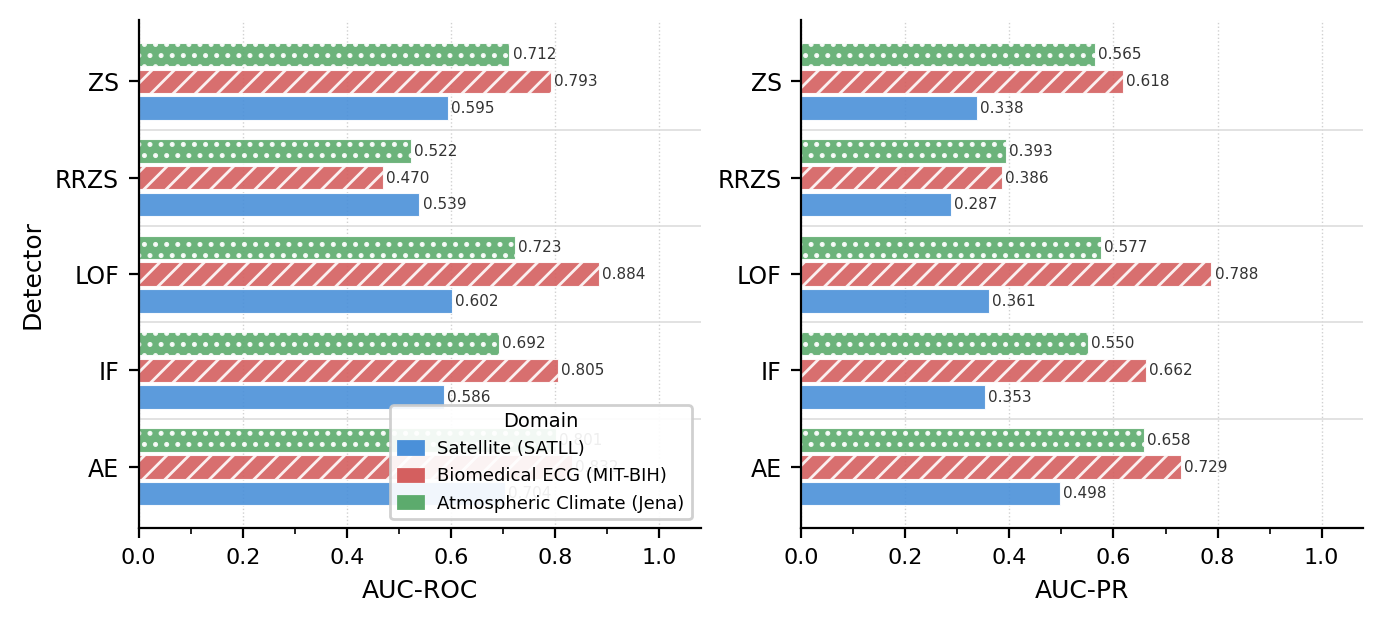
\includegraphics[width=\columnwidth]{figures/fig_domain_comparison.png}
\caption{Cross-domain detection performance (AUC-ROC and AUC-PR) for all five E2
         detectors across satellite (SATLL), biomedical ECG (MIT-BIH), and atmospheric
         climate (Jena). Values are macro-averaged over all sessions per domain.
         AE=Autoencoder, IF=IsolationForest, RRZS=RobustRollingZScore, ZS=ZScore.
         LOF leads on ECG; the Autoencoder leads on satellite and climate.
         AUC-PR is uniformly lower than AUC-ROC, reflecting the $\approx\!20$--$40\%$
         anomaly prevalence across injected variants.}
\label{fig:crossdomain}
\end{figure}

\subsection{Semantic Knowledge Graph}

A four-family satellite M4 run produces a knowledge graph with 869 nodes and
11,762 edges. The top SPARQL-queried evidence class is
\texttt{sat:AttitudeDeterminationAndControlSubsystem}, consistent with the
ADCS-heavy fault taxonomy. Fig.~\ref{fig:kgsubgraph} illustrates the resulting
subgraph. The \texttt{if:featureImportance} predicate supports queries of the form
\texttt{SELECT ?feat ?cls WHERE \{?feat if:evidenceForClass ?cls\}} without
rerunning the detector, enabling post-hoc subsystem attribution. For ECG and
Climate, per-session M4 runs produce lightweight knowledge graphs linking feature
importances to ontology classes via the same interface.

\begin{figure}[t]
\centering
\includegraphics[width=\columnwidth]{figures/fig_kg_subgraph.png}
\caption{M4 knowledge graph subgraph for the satellite domain (AccelerometerTest
         family). Nodes represent OWL class instances (\texttt{sat:ADCS},
         \texttt{sat:OBDH}, etc.), anomaly tags, and IsolationForest feature nodes.
         Edges carry \texttt{if:featureImportance} and \texttt{if:evidenceForClass}
         predicates, enabling SPARQL queries that link detector evidence to satellite
         engineering subsystems without re-executing the detector.}
\label{fig:kgsubgraph}
\end{figure}

\subsection{Runtime Characterisation}

Table~\ref{tab:runtime} gives per-module wall-clock times measured on a standard
laptop (Apple M-series, single thread). E2 accounts for roughly 80--90\% of total
pipeline time; a detector-fit cache---keyed on detector configuration rather than
fault tag---ensures each family incurs exactly one training pass and re-evaluates
all $N_{\text{faults}} \times 3 \times 2$ variants without redundant model
refits. Correcting a prior defect that re-trained all five detectors once per fault
tag ($6\times$ redundant Autoencoder fits per record) reduced ECG E2 time from
$>\!1{,}000$\,s per record to the values shown. Core modules M1--M5 together consume
less than 10\% of runtime, confirming that framework overhead is negligible relative
to domain analysis costs. M3 remains under 1\,s across all domains thanks to the
Cython-compiled skew/kurtosis accumulator and the batched stride-tricks FFT.

SensorWF targets offline analysis of archived sensor sessions rather than
real-time streaming; all data volumes fit comfortably in memory on standard hardware
(peak: $\sim$100\,MB for the satellite combined feature matrix).

\begin{table}[t]
\caption{Per-Module Runtime (Satellite, 4 Families, 2 Variants, 3 Tiers)}
\label{tab:runtime}
\centering
\scriptsize
\setlength{\tabcolsep}{3.5pt}
\begin{tabular}{@{}lrrl@{}}
\toprule
\textbf{Module} & \textbf{Time (s)} & \textbf{\%} & \textbf{Notes} \\
\midrule
M1 Ingestion     & $<$1     & $<$1  & Parse SCOTTI archive \\
M2 Quality       & $<$1     & $<$1  & Clean + flag channels \\
M3 Features      & $<$1     & $<$1  & 9 families; Cython O($n$) + batched FFT \\
E1 Injection     & $\sim$5  & $\sim$1  & Generate 432 labelled CSVs \\
E2 Detection     & $\sim$400 & $\sim$90 & Train 5 ML detectors; config-keyed cache \\
M4 Semantic      & $\sim$30 & $\sim$7  & Build KG from ML evidence + OWL \\
M5 Provenance    & $<$1     & $<$1  & Serialise PROV-O trace + SHA-256 \\
\midrule
Total            & $\sim$440 & 100  & Single laptop, no GPU \\
\bottomrule
\end{tabular}
\end{table}

\subsection{M3 Rolling-Window Sensitivity}

Rolling-window size is the primary hyperparameter in M3. Fig.~\ref{fig:ablation}
shows mean AUC-ROC and AUC-PR on a representative 5-record ECG subset across four
window sizes (15, 30, 50, 100 samples). The Autoencoder and IsolationForest are
relatively insensitive ($\Delta$AUC-ROC $<0.04$), confirming that both exploit
temporal patterns stable across window scales. ZScore and RobustRollingZScore show
higher sensitivity ($\Delta$AUC-ROC $\leq 0.10$): larger windows average out abrupt
changes and reduce recall for short-duration Hard-tier faults. LOF sensitivity
is intermediate ($\Delta$AUC-ROC $<0.05$). Results support the adapter-specified
default of 100 samples (2\,s at 50\,Hz) for ECG as a robust operating point.
Full numeric results are available in the supplementary repository.

\begin{figure}[t]
\centering
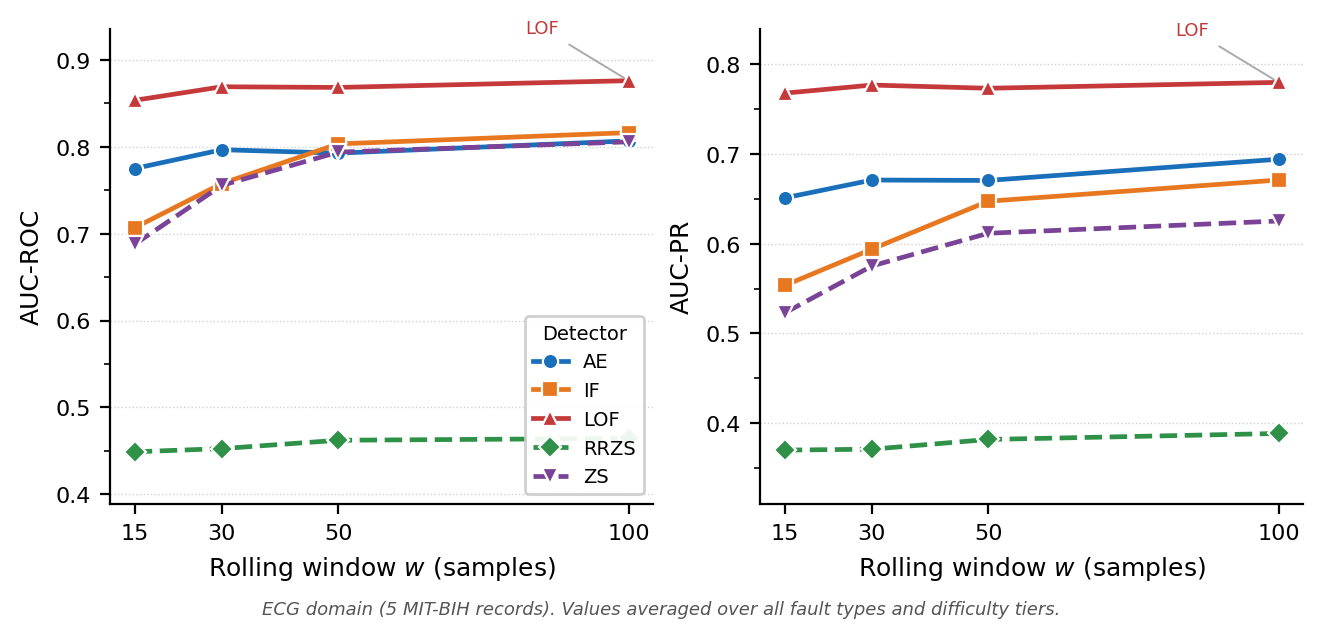
\includegraphics[width=\columnwidth]{figures/fig_ablation_window_ecg.png}
\caption{M3 rolling-window size sensitivity for the ECG domain (5 records, all
         five detectors). AUC-ROC (solid) and AUC-PR (dashed) are plotted for
         window sizes 15, 30, 50, and 100 samples (at 50\,Hz). The Autoencoder and
         IsolationForest are robust to window choice; statistical detectors
         (ZS, RRZS) degrade with larger windows for short Hard-tier faults.}
\label{fig:ablation}
\end{figure}

%% =========================================================
\section{Discussion}
\label{sec:discussion}
%% =========================================================

\subsection{Generalizability and Adapter Effort}

For the three validated domains, implementing each adapter required approximately
150--200 lines of Python; M2--M5 required no code modifications. The component
registry enables programmatic composition: a consumer queries \texttt{components.json}
for modules with a given \texttt{domain\_tag} and receives fully specified I/O
contracts, enabling automated workflow instantiation and validation. The claim that
\emph{only M1 is domain-specific} holds at the code level but warrants a practical
qualification: M2--M5 behaviour depends on adapter-supplied configuration
dictionaries that themselves encode domain knowledge the adapter author must provide
explicitly. Portability limitations---e.g., M2 assumes temporally regular
sampling; irregular-rate or event-driven streams require time-indexed rolling
windows in M3 and resampling extensions in M2---are documented as
\texttt{sensorwf:hasAssumption} predicates in the registry.

\subsection{FAIR Assessment}

Table~\ref{tab:fair} assesses SensorWF against the four FAIR dimensions.
Reproducibility is guaranteed at the code level: running any domain entry point
with \texttt{--seed 42} produces bit-identical CSVs, injection summaries, metrics,
and KG artefacts. The only run-variant output is \texttt{provenance.ttl}, whose
timestamps differ by design. Workflow registration on WorkflowHub with RO-Crate
metadata and immutable Zenodo archives are planned for the open scientific object
release.

\begin{table}[t]
\caption{SensorWF FAIR Assessment}
\label{tab:fair}
\centering
\scriptsize
\setlength{\tabcolsep}{3pt}
\begin{tabular}{@{}lp{5.4cm}@{}}
\toprule
\textbf{Principle} & \textbf{SensorWF Implementation} \\
\midrule
\textbf{Findable}      & \texttt{components.json} registry; SHA-256-checksummed provenance published with code; DOI via Zenodo (planned) \\
\textbf{Accessible}    & Open formats: CSV, JSON, RDF/Turtle, OWL; three public benchmark datasets; self-contained per-domain HTML run report (quality tables, aggregated ML results, embedded figures, live KG visualisation) \\
\textbf{Interoperable} & PROV-O + ProvONE; SSN/SOSA-aligned OWL; standardised DataFrame schema; typed module contracts \\
\textbf{Reusable}      & Domain assumptions encoded in machine-readable component registry; any sensor domain can be integrated without altering the analytical core; \texttt{DomainAdapter} interface; seeded RNG; \texttt{--rerun} cache bypass; \texttt{sensorwf:hasAssumption} predicates \\
\bottomrule
\end{tabular}
\end{table}

\subsection{Relation to Satellite Anomaly Benchmarks}

The ESA-ADB benchmark \cite{esa_adb2024} recommends event-level ground truth,
affiliation-aware scoring, and dynamic/EVT thresholding with postprocessing for
operational satellite telemetry. OPS-SAT \cite{ruszczak2025opssat} emphasises
segment-level precision at low operating FPR. SensorWF partially addresses these
recommendations: density-based detectors (IF, LOF) use POT EVT calibration
(Section~\ref{sec:protocol}), and an event-level \texttt{event\_detected} metric is
emitted per variant. Full affiliation-aware scoring and dynamic postprocessing remain
priority extensions. E2's threshold strategy and detector suite are registry-declared
parameters, facilitating incremental alignment with ESA-ADB protocols without
modifying any core module.

\subsection{Limitations}

\textbf{Synthetic-only evaluation.} All ground-truth labels are generated by E1;
no real annotated anomalies are used. This risks overstating generality relative to
operational benchmark performance (e.g., ESA-ADB, OPS-SAT). Evaluation on real
annotated datasets is a priority extension.

\textbf{Sample-wise metrics.} AUC-ROC and AUC-PR are computed at the sample level;
the binary \texttt{event\_detected} flag adds an event-level complement per variant.
Event-wise, affiliation-aware, and range-based metrics \cite{esa_adb2024} better
reflect detection quality for operational use and are identified as a priority
extension.

\textbf{Deep learning baselines.} The five E2 detectors do not include
transformer-based approaches such as iTransformer \cite{itransformer2024} or
TranAD \cite{tuli2022tranad}, which require separate deep learning frameworks.
The registry-based E2 architecture accommodates these; integrating at least one
transformer baseline is planned as the immediate next step.

\textbf{Provenance completeness.} SHA-256 checksums are computed automatically
for all file-path entities and stored as \texttt{telwf:sha256} triples, enabling
bit-level reproducibility verification. Ontology class mappings have not been
externally validated by domain experts; the current lexical prefix-matching
heuristic is a practical approximation pending expert review.

%% =========================================================
\section{Conclusion}
\label{sec:conclusion}
%% =========================================================

SensorWF demonstrates that a FAIR-annotated, generalizable workflow framework for
scientific sensor time-series analysis is both tractable and practically useful
across disciplinary boundaries. Separating domain-specific ingestion (M1 adapter)
from a reusable analytical core (M2--M5) and encoding domain assumptions in a
machine-readable component registry---so that any sensor domain can be integrated
and reused without altering the analytical core---lets researchers adopt, adapt,
and extend a common pipeline without per-domain reimplementation. Use-case
extensions (E1 fault injection, E2 anomaly detection) attach to core typed outputs
without modifying any core module, demonstrating that the architecture supports
diverse downstream analyses.

Cross-domain validation across spacecraft telemetry (4 SATLL families), ambulatory
ECG (20 MIT-BIH records spanning all major rhythm classes), and atmospheric climate
(7 Jena half-year sessions) shows that a consistent detection architecture
emerges from a single codebase with domain-specific configuration exclusively in M1.
The Autoencoder leads on satellite (AUC-ROC $0.704$) and climate ($0.801$); LOF,
a density-based detector evaluated here across all three domains, achieves the
highest AUC-ROC ($0.884\pm0.035$) and AUC-PR ($0.788\pm0.077$) on the 20-record
ECG benchmark. EVT-calibrated thresholding for density-based detectors,
rolling-window sensitivity analysis, and an event-level detection metric
strengthen the evaluation protocol. Key remaining limitations---synthetic-only
evaluation, point-wise metrics, and the absence of transformer baselines---are
explicitly documented as \texttt{sensorwf:hasAssumption} predicates. KISPE SATLL
data and all code will be released on GitHub as an open scientific object.

%% =========================================================
\section*{Acknowledgment}
%% =========================================================

The authors thank KISPE Space Systems for access to the SATLL telemetry datasets,
PhysioNet for the MIT-BIH Arrhythmia Database, and the Max Planck Institute for
Biogeochemistry for the Jena Climate Dataset. Portions of this manuscript were
drafted with the assistance of an AI language model (Claude, Anthropic); all
scientific content, results, and conclusions were verified and approved by the authors.

%% =========================================================

\bibliographystyle{IEEEtran}
\bibliography{main}

%% =========================================================
\appendices
%% =========================================================

\section{Satellite Detection Performance by Difficulty Tier}
\label{app:tier}

Table~\ref{tab:tier} disaggregates the satellite AUC-ROC and AUC-PR results
(averaged across four families) by the three E1 difficulty tiers.
Hard-tier faults produce higher AUC-ROC than medium-tier for most detectors,
confirming the non-monotone difficulty ordering discussed in Section~\ref{sec:eval}.
AUC-PR generally increases with tier difficulty because the injected anomaly
windows occupy a larger fraction of the evaluation set under hard-tier
duration scaling, reducing effective imbalance.

\begin{table}[h]
\caption{Satellite AUC-ROC / AUC-PR by Difficulty Tier (4 Families, 18 Fault Types)}
\label{tab:tier}
\centering
\scriptsize
\setlength{\tabcolsep}{2.5pt}
\begin{tabular}{@{}llrrrrr@{}}
\toprule
\textbf{Tier} & \textbf{Det.} & \textbf{AUC-ROC} & \textbf{AUC-PR} & \textbf{Recall} & \textbf{FPR} & \textbf{F1} \\
\midrule
Easy   & AE   & \textbf{0.764} & 0.423 & 0.78 & 0.47 & 0.23 \\
       & IF   & 0.635 & 0.239 & 0.34 & 0.20 & 0.16 \\
       & LOF  & 0.649 & 0.256 & 0.37 & 0.18 & 0.19 \\
       & RRZS & 0.547 & 0.140 & 0.17 & 0.15 & 0.08 \\
       & ZS   & 0.620 & 0.200 & 0.18 & 0.13 & 0.08 \\
\midrule
Medium & AE   & \textbf{0.663} & 0.479 & 0.72 & 0.52 & 0.38 \\
       & IF   & 0.544 & 0.337 & 0.30 & 0.22 & 0.22 \\
       & LOF  & 0.570 & 0.344 & 0.32 & 0.21 & 0.25 \\
       & RRZS & 0.527 & 0.291 & 0.14 & 0.15 & 0.12 \\
       & ZS   & 0.588 & 0.347 & 0.16 & 0.15 & 0.12 \\
\midrule
Hard   & AE   & \textbf{0.685} & \textbf{0.592} & 0.73 & 0.48 & 0.52 \\
       & IF   & 0.580 & 0.483 & 0.29 & 0.22 & 0.27 \\
       & LOF  & 0.586 & 0.483 & 0.31 & 0.19 & 0.30 \\
       & RRZS & 0.543 & 0.431 & 0.16 & 0.15 & 0.15 \\
       & ZS   & 0.576 & 0.466 & 0.17 & 0.17 & 0.14 \\
\bottomrule
\multicolumn{7}{l}{\scriptsize AE=Autoencoder, IF=IsolationForest, RRZS=RobustRollingZScore, ZS=ZScore.} \\
\multicolumn{7}{l}{\scriptsize Bold: best AUC-ROC and AUC-PR per tier. Averaged across 4 families.}
\end{tabular}
\end{table}

\section{M4 Knowledge Graph SPARQL Query Examples}
\label{app:sparql}

The following queries illustrate the post-hoc analytical value of the M4
knowledge graph without re-executing any ML detector.

\noindent\textbf{Q1: Which satellite subsystems carry the strongest anomaly evidence?}
\begin{lstlisting}[basicstyle=\ttfamily\scriptsize]
PREFIX if: <http://sensorwf.org/interpretability#>
PREFIX sat: <http://sensorwf.org/satellite#>
SELECT ?subsystem (SUM(?imp) AS ?total_evidence)
WHERE {
  ?feat if:belongsToSubsystem ?subsystem ;
        if:featureImportance ?imp .
}
GROUP BY ?subsystem ORDER BY DESC(?total_evidence)
\end{lstlisting}

\noindent\textbf{Q2: Top-5 features by IsolationForest importance for gyro faults:}
\begin{lstlisting}[basicstyle=\ttfamily\scriptsize]
PREFIX if: <http://sensorwf.org/interpretability#>
SELECT ?feat ?cls ?imp
WHERE {
  if:tag:A2_gyro_clipping if:importantFeature ?feat .
  ?feat if:featureImportance ?imp ;
        if:mapsToSensorClass ?cls .
}
ORDER BY DESC(?imp) LIMIT 5
\end{lstlisting}

These queries execute against the RDF/Turtle graph
(\texttt{if\_ontology\_graph.ttl}) produced by M4 using any SPARQL~1.1
endpoint (e.g., Apache Jena Fuseki, RDFLib). No Python or ML libraries are
required for post-hoc subsystem attribution.

\section{M3 Rolling-Window Ablation -- Full Numeric Results}
\label{app:ablation}

Table~\ref{tab:ablation_full} gives the complete per-detector AUC-ROC and
AUC-PR values underlying Fig.~\ref{fig:ablation}. Results are averaged over
all fault types and three difficulty tiers for 5 MIT-BIH ECG records.

\begin{table}[h]
\caption{M3 Window Ablation -- Mean AUC-ROC / AUC-PR (ECG, 5 Records)}
\label{tab:ablation_full}
\centering
\scriptsize
\setlength{\tabcolsep}{3pt}
\begin{tabular}{@{}lrrrrr@{}}
\toprule
 & \multicolumn{5}{c}{\textbf{AUC-ROC (AUC-PR)}} \\
\cmidrule{2-6}
$w$ & \textbf{AE} & \textbf{IF} & \textbf{LOF} & \textbf{RRZS} & \textbf{ZS} \\
\midrule
  15 & 0.775 (0.651) & 0.707 (0.554) & 0.854 (0.768) & 0.449 (0.370) & 0.688 (0.523) \\
  30 & 0.797 (0.671) & 0.758 (0.594) & 0.869 (0.777) & 0.452 (0.371) & 0.756 (0.575) \\
  50 & 0.793 (0.671) & 0.803 (0.647) & 0.868 (0.773) & 0.462 (0.382) & 0.794 (0.612) \\
 100 & 0.807 (0.694) & 0.816 (0.671) & 0.876 (0.780) & 0.464 (0.388) & 0.806 (0.625) \\
\bottomrule
\end{tabular}
\end{table}

\end{document}
